\documentclass[11pt, a4paper]{article}
\usepackage[margin=2.4cm]{geometry}
\usepackage[T1]{fontenc}
\usepackage{lmodern}          % Type 1 vector fonts
\usepackage{cmap}             % ToUnicode CMap -> copyable text and accents
\usepackage[utf8]{inputenc}
\usepackage[english]{babel}
\usepackage{amsmath, amssymb, amsthm}
\usepackage{bm}
\usepackage{mathtools}
\usepackage{enumitem}
\usepackage{booktabs}
\usepackage{array}
\usepackage{xcolor}
\usepackage{titlesec}
\usepackage{parskip}
\usepackage{hyperref}
\usepackage{fancyhdr}
\usepackage{tcolorbox}
\usepackage{graphicx}
\usepackage{caption}
\tcbuselibrary{skins, breakable}

\definecolor{darkblue}{RGB}{15,55,115}
\definecolor{midblue}{RGB}{30,100,180}
\definecolor{theorybg}{RGB}{245,250,255}
\definecolor{questionbg}{RGB}{255,252,240}
\definecolor{evencolor}{RGB}{60,0,100}
\definecolor{rubricbg}{RGB}{248,246,252}
\definecolor{planbg}{RGB}{246,252,247}
\definecolor{plancolor}{RGB}{20,95,55}
\definecolor{trapbg}{RGB}{255,247,245}
\definecolor{trapcolor}{RGB}{150,35,35}

\hypersetup{colorlinks=true, linkcolor=darkblue, urlcolor=midblue,
  pdftitle={Solutions --- Problem Set 5 --- Macroeconomics I MPE Insper},
  pdfauthor={Macroeconomia I --- MPE Insper 2026/T3}}

\setlength{\headheight}{14pt}
\pagestyle{fancy}
\fancyhf{}
\renewcommand{\headrulewidth}{0.4pt}
\fancyhead[L]{\small\textcolor{darkblue}{\textit{Macroeconomia I --- MPE Insper --- 2026/T3}}}
\fancyhead[R]{\small\textcolor{darkblue}{\thepage}}
\fancyfoot[C]{\small\textcolor{gray}{Solutions --- Problem Set 5}}

\titleformat{\section}[block]
  {\large\bfseries\color{darkblue}}{}{0pt}{}
  [\vspace{2pt}\color{darkblue}\rule{\textwidth}{1.5pt}\vspace{4pt}]

\tcbset{
  theorybox/.style={
    enhanced, breakable, colback=theorybg, colframe=darkblue,
    fonttitle=\bfseries\small, coltitle=white, boxrule=0.5pt, arc=3pt,
    left=6pt, right=6pt, top=4pt, bottom=4pt,
  },
  questionbox/.style={
    enhanced, breakable, colback=questionbg, colframe=gray!60,
    fonttitle=\bfseries\small, coltitle=black, boxrule=0.4pt, arc=2pt,
    left=6pt, right=6pt, top=4pt, bottom=4pt, title={\textit{Question}},
  },
  rubricbox/.style={
    enhanced, breakable, colback=rubricbg, colframe=evencolor!70,
    fonttitle=\bfseries\small, coltitle=white, boxrule=0.4pt, arc=2pt,
    left=6pt, right=6pt, top=4pt, bottom=4pt, title={Where the marks are},
  },
  planbox/.style={
    enhanced, breakable, colback=planbg, colframe=plancolor,
    fonttitle=\bfseries\small, coltitle=white, boxrule=0.5pt, arc=3pt,
    left=6pt, right=6pt, top=4pt, bottom=4pt,
  },
  trapbox/.style={
    enhanced, breakable, colback=trapbg, colframe=trapcolor!75,
    fonttitle=\bfseries\small, coltitle=white, boxrule=0.4pt, arc=2pt,
    left=6pt, right=6pt, top=4pt, bottom=4pt,
  },
}

\newcommand{\passo}[1]{\medskip\noindent\textbf{#1}\par\nobreak}
\newcommand{\intuicao}[1]{%
  \medskip\noindent\textcolor{midblue}{\textbf{Economic reading.}} #1\par}
\newcommand{\resp}[1]{%
  \ifmmode {\color{darkblue}#1}\else\textcolor{darkblue}{\textbf{#1}}\fi}
\newcommand{\stst}{^{\ast}}
\newcommand{\MRS}{\mathrm{MRS}}
\newcommand{\MRT}{\mathrm{MRT}}
\newcommand{\Kb}{\bar K}

\setlist[enumerate,1]{label=(\alph*), itemsep=6pt, parsep=2pt, leftmargin=1.6em}
\setlist[itemize,1]{itemsep=3pt, parsep=1pt, leftmargin=1.3em, topsep=3pt}

\begin{document}

%======================================================================
\begin{center}
{\LARGE\bfseries\color{darkblue} Solutions --- Problem Set 5\par}
\vspace{4pt}
{\large MACROECONOMIA 1 --- MPE Insper --- Prof.\ Pedro G.\ Duarte\par}
\vspace{2pt}
{\normalsize 2026, 3\textordmasculine{} trimestre \quad$\cdot$\quad Due: 08/09/2026\par}
\vspace{2pt}
{\small General Equilibrium --- Kurlat (2020), ch.\ 9\par}
\end{center}
\vspace{6pt}

\begin{tcolorbox}[theorybox, title={How to read this document}]
\small
Two questions, and the professor has built them as \textbf{mirror images}. Question 1 is
chapter 9 with \textbf{capital frozen}: no investment technology, $K$ fixed at $\Kb$,
$\delta=0$. Question 2 is chapter 9 with \textbf{labour frozen}: $L_t=1$, no leisure in
preferences. Between them they cover the whole chapter, one margin at a time. Neither is
asking for the full three-agent model in one go, so each demands that you be very clean
about the margin it left switched on.

\smallskip
\textbf{The thread that joins them.} In both, the object that has to be pinned down is a
\emph{price that nothing else determines}. In Question 1 the interest rate cannot move any
goods --- there is no storage and no investment --- so $r$ is purely the price that
reconciles the household to a consumption path it cannot alter. In Question 2 the interest
rate is tied to the marginal product of capital by arbitrage, and the steady state forces
it back to pure impatience. \emph{Preferences fix the interest rate; technology fixes the
quantity of capital.}

\smallskip
Highlighted answers are in \resp{blue}. \textcolor{trapcolor}{\textbf{Red}} boxes are
traps; \textcolor{plancolor}{\textbf{green}} boxes are method. Every number is reproduced
by \texttt{Resolucao/lista5\_codigo/}, which checks each analytical formula against an
independent numerical route and aborts on any mismatch.

\smallskip
\emph{Language.} Written in English, per the project's global output-language rule --- and
in any case the problem set itself is set in English.
\end{tcolorbox}

\begin{center}
\small
\begin{tabular}{@{}lcl@{}}
\toprule
\textbf{Question} & \textbf{Points} & \textbf{Basis in Kurlat} \\
\midrule
1 --- Two periods, fixed capital & 5 & \S9.1--9.2; the machinery of Ex.\ \textbf{9.5}, \textbf{9.7} \\
2 --- Infinite horizon, fixed labour & 5 & \S9.3; Ex.\ \textbf{9.11}, \textbf{9.12}; (e) is Ex.\ \textbf{9.12}'s punchline \\
\bottomrule
\end{tabular}
\end{center}

%======================================================================
\section{Question 1 \quad Two periods, capital fixed at $\Kb$}
%======================================================================

\begin{tcolorbox}[planbox, title={Read the amputation before writing anything}]
\small
Three things are \textbf{gone} relative to Kurlat's \S9.1, and each one removes a line you
would otherwise be expected to write:
\begin{itemize}
\item \textbf{No investment firm.} There is no investment technology at all, so the third
      agent of ch.\ 9 does not exist and equation (9.1.11), $1+r=r^K_2$, has no analogue.
\item \textbf{No capital accumulation.} Equation (9.1.5) is replaced by $K_t=\Kb$ for
      both $t$. And $\delta=0$.
\item \textbf{No storage.} Therefore goods market clearing carries \emph{no investment
      term}: $c_t=F(\Kb,L_t)$, period by period. This single line drives everything below.
\end{itemize}
What survives is exactly two margins: consumption against leisure \emph{within} a period,
and consumption today against consumption tomorrow \emph{across} periods.
\end{tcolorbox}

\subsection*{Item (a) --- the two problems, and why $\Pi=0$}

\passo{The household.}
\[
\max_{c_1,l_1,c_2,l_2}\;\; u(c_1)+v(l_1)+\beta\big[u(c_2)+v(l_2)\big],
\qquad u(c)=\frac{c^{1-\sigma}}{1-\sigma},\quad v(l)=\psi\ln l,
\]
subject to a budget constraint --- and the constraint should be \textbf{built, not quoted}.

\passo{Building (1.1) out of the two period constraints.} The household trades a
one-period bond $a$ ($a>0$ means it lends, $a<0$ that it borrows), bought at date~1 and
repaid with interest at date~2. Period by period, income must cover spending:
\[
\text{date 1:}\quad c_1+a=w_1(1-l_1)+r^K_1\Kb+\Pi_1 ,
\qquad
\text{date 2:}\quad c_2=w_2(1-l_2)+r^K_2\Kb+\Pi_2+(1+r)a .
\]
Two remarks on the second one. The household ends with \textbf{nothing}: there is no
date~3, so leaving assets behind would be strictly wasteful ($u$ is increasing), and
leaving debt behind is not permitted. And $\Kb$ appears only through its \emph{rent} at
both dates, never as a principal --- see the red box below.

Now divide the date-2 constraint by $1+r$ and add it to the date-1 one. The $a$ terms are
$+a$ and $-\frac{(1+r)a}{1+r}=-a$, so they \textbf{cancel}:
\[
\boxed{\;c_1+\frac{c_2}{1+r}\;=\;w_1(1-l_1)+\frac{w_2(1-l_2)}{1+r}
\;+\;r^K_1\Kb+\frac{r^K_2\Kb}{1+r}\;+\;\Pi\;},
\qquad \Pi\equiv\Pi_1+\frac{\Pi_2}{1+r} .
\tag{1.1}
\]

\begin{tcolorbox}[planbox, title={Where the bond went --- and why item (b) has only one $\lambda$}]
\small
$a$ vanished from (1.1), and that is the whole content of ``there is a credit market''.
Borrowing is not a separate decision to be optimised: once $c_1$ and $l_1$ are chosen, the
date-1 constraint \emph{defines} what $a$ must be,
\[
a=w_1(1-l_1)+r^K_1\Kb+\Pi_1-c_1 ,
\]
and since $a$ never enters the utility function, the household cares about the consumption
path and is indifferent to how it is financed. \textbf{Two constraints became one, which is
exactly why there will be one multiplier and not two} in item (b) --- and why the Euler
equation exists at all. Without credit, $a\equiv0$ would be forced, the two constraints
would stay separate, and the household would be stuck consuming its income date by date.

\smallskip
In \emph{equilibrium} $a=0$ anyway --- a representative household has nobody to trade with
--- but that is a conclusion, not an assumption. The household is free to borrow; $r$ moves
until it does not want to. See item (c).
\end{tcolorbox}

\begin{tcolorbox}[trapbox, title={The one place this differs from Kurlat (9.1.1)}]
\small
Kurlat's household holds $\Kb\big(1+r^K_1-\delta\big)$, which includes the \textbf{principal}
because in his model capital can be sold into the used-capital market. \textbf{Here it
cannot.} There is no investment technology, so no market exists in which a unit of capital
could be turned back into consumption goods. The household can only \emph{rent} it out, and
it does so in both periods. Hence rental income only, $r^K_1\Kb$ and $r^K_2\Kb$, and no
$(1-\delta)$ term anywhere. Say this explicitly in your answer --- writing Kurlat's term
here imports a market this economy does not have.
\end{tcolorbox}

\passo{The firm, separately in each period $t=1,2$.}
\[
\Pi^F_t=\max_{K_t,\,L_t}\;\; A_t K_t^{\alpha}L_t^{1-\alpha}-w_tL_t-r^K_tK_t
\tag{1.2}
\]
The firm is \textbf{static}: it rents everything period by period and carries nothing
between dates, so it has no discount factor and no intertemporal problem.

\passo{Why profit is zero.} Because $F$ has \textbf{constant returns to scale} and factors
are paid their marginal products. The Cobb--Douglas exponents sum to one, so $F$ is
homogeneous of degree one and Euler's theorem gives
\[
F(K,L)=K\,F_K+L\,F_L .
\]
Verify it directly: $F_K=\alpha F/K$ and $F_L=(1-\alpha)F/L$, so
$K F_K+L F_L=\alpha F+(1-\alpha)F=F$. \checkmark\ Now impose the firm's first-order
conditions $F_K=r^K_t$ and $F_L=w_t$:
\[
r^K_t K_t+w_t L_t=\alpha F+(1-\alpha)F=F(K_t,L_t)
\qquad\Longrightarrow\qquad
\resp{\Pi^F_t=0 .}
\]
Revenue exactly exhausts factor payments. \checkmark\ (checked in
\texttt{l5q1.py::check\_zero\_lucro}).

\intuicao{This is not an equilibrium condition that has to be imposed --- it is an
\emph{identity} that follows from constant returns plus competitive pricing. Its role is to
let $\Pi$ drop out of (1.1), so that in equilibrium household wealth is just labour income
plus rental income. Note also that it is \emph{scale} that delivers zero profit, not
$\alpha$: any constant-returns technology would do.}

\subsection*{Item (b) --- the first-order conditions}

\passo{Step 1 --- the Lagrangian.} Write the right-hand side of (1.1) as \textbf{wealth},
\[
W(l_1,l_2)\;\equiv\;w_1(1-l_1)+\frac{w_2(1-l_2)}{1+r}
\;+\;r^K_1\Kb+\frac{r^K_2\Kb}{1+r}\;+\;\Pi ,
\]
keeping the arguments visible: an hour of leisure at date $t$ costs $w_t$ of wealth, and
that is the only reason a wage will appear in the leisure condition below. The constraint
holds with \textbf{equality} because $u$ is strictly increasing --- the household never
ends up holding unspent wealth --- so we may attach a single multiplier $\lambda$ to it:
\[
\mathcal{L}\;=\;\underbrace{u(c_1)+v(l_1)+\beta\big[u(c_2)+v(l_2)\big]}_{\text{measured in utils}}
\;+\;\lambda\underbrace{\Big[\,W(l_1,l_2)-c_1-\tfrac{c_2}{1+r}\,\Big]}_{\text{measured in date-1 goods}} .
\]
The two braces are in \textbf{different units}. $\lambda$ is the exchange rate between
them, and everything below is bookkeeping.

\passo{Step 2 --- differentiate.} Four choice variables, four conditions:
\[
\frac{\partial\mathcal{L}}{\partial c_1}=u'(c_1)-\lambda=0,
\qquad
\frac{\partial\mathcal{L}}{\partial c_2}=\beta u'(c_2)-\frac{\lambda}{1+r}=0,
\]
\[
\frac{\partial\mathcal{L}}{\partial l_1}=v'(l_1)-\lambda w_1=0,
\qquad
\frac{\partial\mathcal{L}}{\partial l_2}=\beta v'(l_2)-\frac{\lambda w_2}{1+r}=0,
\]
that is,
\[
\underbrace{u'(c_1)=\lambda}_{\text{(i)}},\qquad
\underbrace{\beta u'(c_2)=\frac{\lambda}{1+r}}_{\text{(ii)}},\qquad
\underbrace{v'(l_1)=\lambda w_1}_{\text{(iii)}},\qquad
\underbrace{\beta v'(l_2)=\frac{\lambda w_2}{1+r}}_{\text{(iv)}} .
\]
Every one of the four reads the same sentence: \emph{marginal utility of the thing}
$=\lambda\times$ \emph{what one unit of that thing costs, priced in date-1 goods}. A unit
of $c_1$ costs $1$; a unit of $c_2$ costs $\tfrac{1}{1+r}$, because that is what must be
set aside today to have one good tomorrow; an hour of leisure costs the wage $w_t$,
discounted if it falls at date~2.

Notice the asymmetry that will produce the Euler equation: $\beta$ sits on the
\textbf{utility} side and is the household's own impatience, while $\tfrac{1}{1+r}$ sits
on the \textbf{price} side and is the market's. Optimality is the point where the two are
reconciled.

\begin{tcolorbox}[planbox, title={What $\lambda$ is --- three readings of the same number}]
\small
\textbf{1. Mechanically, a unit converter.} The objective is in utils, the constraint in
date-1 goods. You cannot set one equal to the other, so the first-order conditions need a
conversion factor. $\lambda$ carries the units \emph{utils per date-1 good}.

\smallskip
\textbf{2. Economically, the marginal utility of wealth} --- the shadow price of the
budget constraint. Let $V(W)$ be maximised lifetime utility as a function of wealth. The
envelope theorem gives
\[
\lambda=V'(W),
\]
so $\lambda$ answers the question: \emph{hand this household one more unit of date-1
goods --- by how much does its lifetime utility rise?} A poor household has a large
$\lambda$, a rich one a small $\lambda$.

\smallskip
\textbf{3. Concretely, here it \emph{equals} $u'(c_1)$.} Condition (i) says precisely that:
\[
\lambda=u'(c_1)=c_1^{-\sigma}>0 .
\]
Positive, which confirms the constraint binds. And it is no accident: the budget was
written in \textbf{date-1 goods}, and the household can always turn one unit of date-1
wealth into one unit of $c_1$, so the value of wealth \emph{must} come out equal to the
marginal utility of present consumption. Write the same constraint in date-2 units and the
multiplier comes out as $\beta u'(c_2)$ instead. The number moves with the numeraire; the
economics does not. \resp{$\lambda$ is a price, not a preference parameter.}

\smallskip
\textbf{Counting.} Five unknowns ($c_1,c_2,l_1,l_2,\lambda$) against five equations (the
four conditions plus the constraint itself). $\lambda$ \emph{is} determined --- it is
simply not needed for the two boxed results, because both are ratios.
\end{tcolorbox}

\begin{tcolorbox}[trapbox, title={Why there is \emph{one} $\lambda$ and not two --- the credit market is hiding in here}]
\small
There is one multiplier because there is one constraint, and there is one constraint
because the household \textbf{can borrow and lend at $r$}. That is exactly what licenses
collapsing the two period budgets into the single present-value constraint (1.1).

\smallskip
Suppose credit were unavailable, so the household had to satisfy
\[
c_1\le w_1(1-l_1)+r^K_1\Kb
\qquad\text{and}\qquad
c_2\le w_2(1-l_2)+r^K_2\Kb
\]
\emph{separately}. Then there would be two multipliers, $\lambda_1$ and $\lambda_2$, the
consumption conditions would read $u'(c_1)=\lambda_1$ and $\beta u'(c_2)=\lambda_2$, and
dividing one by the other would give
\[
\frac{u'(c_1)}{\beta u'(c_2)}=\frac{\lambda_1}{\lambda_2}\;\neq\;1+r
\quad\text{in general.}
\]
\textbf{No Euler equation.} The Euler equation is not a law of nature --- it is the
footprint of a market. Seeing that the \emph{same} $\lambda$ appears at both dates
\emph{is} seeing that the household can move goods through time at the price $1+r$.
(This is the same point as the credit-limit exercise in ch.\ 6: bind the household and the
Euler equation becomes an inequality.)
\end{tcolorbox}

\passo{Step 3 --- take ratios, and $\lambda$ cancels twice.} $\lambda$ is one number, not
one per date, so any ratio of two of the four conditions is free of it. That is why it
never has to be computed, and why the content of optimality is always a \emph{ratio}: a
marginal rate of substitution set equal to a relative price.

\passo{The \emph{intratemporal} margin --- consumption against leisure.} Dividing the
leisure condition by the consumption condition, in each period separately --- (iii)$/$(i)
at date~1, and (iv)$/$(ii) at date~2, where $\beta$ and $\tfrac{1}{1+r}$ cancel along with
$\lambda$,
\[
\frac{v'(l_1)}{u'(c_1)}=\frac{\lambda w_1}{\lambda}=w_1 ,
\qquad
\frac{\beta v'(l_2)}{\beta u'(c_2)}=\frac{\lambda w_2/(1+r)}{\lambda/(1+r)}=w_2 ,
\]
which is why the same condition holds in both periods and carries no intertemporal price:
\[
\boxed{\;\frac{v'(l_t)}{u'(c_t)}=w_t\;}
\qquad\Longleftrightarrow\qquad
\boxed{\;\frac{\psi\,c_t^{\sigma}}{1-L_t}=w_t\;},\qquad t=1,2.
\tag{1.3}
\]
This is Kurlat (9.1.7). \resp{It is the condition that describes the trade-off between
consumption and leisure.}

\passo{The \emph{intertemporal} margin --- present against future consumption.} Dividing
the $c_1$ condition by the $c_2$ condition, (i)$/$(ii):
\[
\frac{u'(c_1)}{\beta u'(c_2)}=\frac{\lambda}{\lambda/(1+r)}=1+r ,
\]
which rearranges to
\[
\boxed{\;u'(c_1)=\beta(1+r)\,u'(c_2)\;}
\qquad\Longleftrightarrow\qquad
\boxed{\;\left(\frac{c_2}{c_1}\right)^{\sigma}=\beta(1+r)\;}
\tag{1.4}
\]
This is the \textbf{Euler equation}, Kurlat (9.1.8). \resp{It is the condition that
describes the trade-off between present and future consumption.}

\passo{The firm.}
\[
\boxed{\;w_t=(1-\alpha)A_t\Kb^{\alpha}L_t^{-\alpha}=(1-\alpha)\frac{Y_t}{L_t}\;},
\qquad
\boxed{\;r^K_t=\alpha A_t\Kb^{\alpha-1}L_t^{1-\alpha}=\alpha\frac{Y_t}{\Kb}\;}
\tag{1.5}
\]

\begin{tcolorbox}[trapbox, title={$\sigma$ or $1/\sigma$?}]
\small
State it once, explicitly, and you cannot be marked wrong under either convention:
\textbf{$\sigma$ is the curvature of $u$} (the coefficient of relative risk aversion), and
\textbf{$1/\sigma$ is the elasticity of intertemporal substitution}. It matters in item (e),
where the sign of the whole answer turns on $1-\sigma$.
\end{tcolorbox}

\subsection*{Item (c) --- the definition of competitive equilibrium}

A \textbf{competitive equilibrium} is an allocation
$\{c_1,c_2,l_1,l_2,L_1,L_2,K_1,K_2\}$ and a price system
$\{r,\;w_1,w_2,\;r^K_1,r^K_2\}$ such that:

\begin{enumerate}[label=\textbf{\arabic*.}, leftmargin=2em]
\item \textbf{Household optimality.} Given the prices, the allocation solves the utility
      maximisation problem subject to the present-value budget constraint (1.1) --- that
      is, it satisfies (1.3) and (1.4).
\item \textbf{Firm optimality.} Given the prices, in each period the firm's choice of
      $(K_t,L_t)$ solves (1.2) --- that is, it satisfies (1.5).
\item \textbf{Market clearing}, in each period:
\end{enumerate}
\[
\text{goods:}\quad \boxed{\,c_t=A_t\Kb^{\alpha}L_t^{1-\alpha}\,},
\qquad
\text{labour:}\quad \boxed{\,L_t+l_t=1\,},
\qquad
\text{capital:}\quad \boxed{\,K_t=\Kb\,}.
\tag{1.6}
\]

\passo{Why the credit market clears without being listed.} It is worth proving rather than
asserting. Take the household's \emph{date-1} constraint, the one that still contains the
bond, and impose what we already know: $L_1=1-l_1$ from labour clearing, $\Pi_1=0$ from
item (a), and Euler's theorem $w_1L_1+r^K_1\Kb=F(\Kb,L_1)=Y_1$. Then
\[
c_1+a=w_1L_1+r^K_1\Kb+\Pi_1=Y_1 .
\]
Goods clearing says $c_1=Y_1$. Subtracting,
\[
\boxed{\;a=0\;}
\]
\resp{Three markets clearing force the fourth.} That is \textbf{Walras's law}, and it is
why the definition above need not list the credit market: doing so would be redundant, not
wrong. With a representative household there is also a one-line version of the same
conclusion --- \emph{the representative agent cannot trade with itself} --- but the
accounting argument is the one that generalises.

\begin{tcolorbox}[rubricbox]
\small
\textbf{Three things earn the marks here, and all three are easy to drop.}
\begin{itemize}
\item \textbf{All three conditions.} A student who writes only the first-order conditions
      has given \emph{demand}, not equilibrium.
\item \textbf{Goods clearing has no investment term.} $c_t=Y_t$, period by period. This is
      where the amputation shows up, and every result in (d) and (e) descends from it.
\item \textbf{The credit market.} Net lending is zero, $a=0$. Say that it follows from the
      others by \textbf{Walras's law}, and that with a representative household it must
      hold anyway: \emph{the representative agent cannot trade with itself.}
\end{itemize}
\end{tcolorbox}

\subsection*{Item (d) --- equilibrium labour, and the interest rate}

\passo{Step 1: substitute the firm's condition into the household's.} Put $w_t=F_L$ from
(1.5) into (1.3):
\[
\boxed{\;
\underbrace{\frac{v'(l_t)}{u'(c_t)}}_{\textstyle \MRS_{l,c}}
=\underbrace{F_L(\Kb,L_t)}_{\textstyle \MRT_{l,c}}\;}
\tag{1.7}
\]
which is exactly the form the question asks for, and is Kurlat (9.1.12). On the left, the
rate at which the household \emph{is willing} to trade leisure for consumption. On the
right, the rate at which the economy \emph{is able} to convert leisure into consumption ---
which is the marginal product of labour. The wage has cancelled: it appeared once in a
household condition and once in a firm condition.

\passo{Step 2: substitute goods market clearing.} Using $c_t=A_t\Kb^{\alpha}L_t^{1-\alpha}$
and $v'(l_t)=\psi/(1-L_t)$, $u'(c_t)=c_t^{-\sigma}$:
\[
\frac{\psi}{1-L_t}\Big(A_t\Kb^{\alpha}L_t^{1-\alpha}\Big)^{\sigma}
=(1-\alpha)A_t\Kb^{\alpha}L_t^{-\alpha}.
\]
Take the power through on the left, separating the $L_t$ from the rest:
\[
\frac{\psi\,\big(A_t\Kb^{\alpha}\big)^{\sigma}L_t^{(1-\alpha)\sigma}}{1-L_t}
=(1-\alpha)\,A_t\Kb^{\alpha}\,L_t^{-\alpha}.
\]
Now multiply both sides by $L_t^{\alpha}$, which clears the negative exponent on the right
and merges the two powers of $L_t$ on the left into
$L_t^{(1-\alpha)\sigma+\alpha}$; then divide by $\psi\big(A_t\Kb^{\alpha}\big)^{\sigma}$,
which leaves $\big(A_t\Kb^{\alpha}\big)^{1-\sigma}$ on the right:
\[
\boxed{\;
\frac{L_t^{\,\alpha+(1-\alpha)\sigma}}{1-L_t}
=\frac{1-\alpha}{\psi}\Big(A_t\Kb^{\alpha}\Big)^{1-\sigma}\;}
\tag{1.8}
\]

\begin{tcolorbox}[planbox, title={Why (1.8) has exactly one solution --- say this}]
\small
The left-hand side is the product of $L^{\alpha+(1-\alpha)\sigma}$, strictly increasing
from $0$, and $1/(1-L)$, strictly increasing to $+\infty$. So it rises \textbf{strictly
monotonically from $0$ to $+\infty$} on $(0,1)$, while the right-hand side is a positive
constant. Exactly one crossing. \checkmark\ (verified on a grid of $2\times10^5$ points in
\texttt{l5q1.py::check\_unicidade}; panel (i) of Figure~\ref{fig:trab} draws it.)

\smallskip
There is \textbf{no closed form}, and none is expected --- Kurlat's own key to PSET 4 stops
at an implicit equation for exactly this reason. Characterise it and differentiate
implicitly.
\end{tcolorbox}

Note that (1.8) involves only date-$t$ objects. \textbf{The two periods do not interact on
the labour margin at all}, precisely because no goods can be moved between them.

\begin{center}
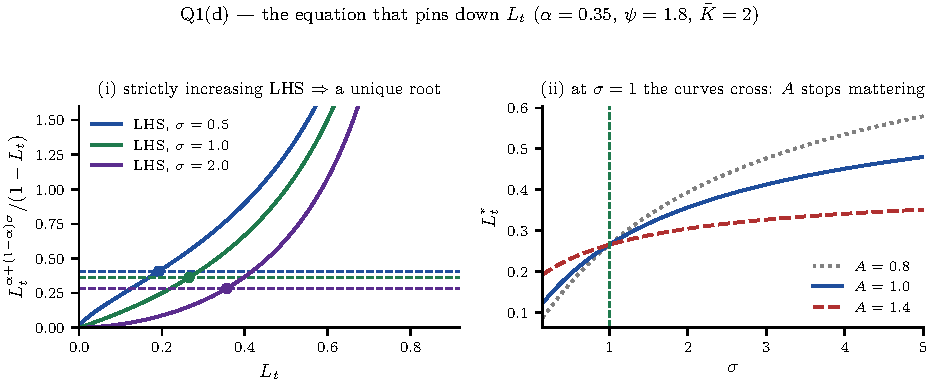
\includegraphics[width=\linewidth]{fig/fig_l5q1_trabalho.pdf}\\[3pt]
\captionof{figure}{Q1(d). Left: the strictly increasing left-hand side of (1.8) against the
constant right-hand side --- one crossing, for every $\sigma$. Right: equilibrium hours
against $\sigma$; at $\sigma=1$ the three curves meet, because productivity drops out of
(1.8).}
\label{fig:trab}
\end{center}

\passo{Step 3: the interest rate.} From the Euler equation (1.4) with goods clearing (1.6):
\[
1+r=\frac{1}{\beta}\left(\frac{c_2}{c_1}\right)^{\sigma},
\qquad
\frac{c_2}{c_1}=\frac{A_2}{A_1}\left(\frac{L_2}{L_1}\right)^{1-\alpha},
\]
so
\[
\boxed{\;1+r=\frac{1}{\beta}
\left[\frac{A_2}{A_1}\left(\frac{L_2}{L_1}\right)^{1-\alpha}\right]^{\sigma}\;}
\tag{1.9}
\]
with $L_1$ and $L_2$ each solving (1.8) at their own $A_t$. \checkmark

\intuicao{Read what (1.9) does \emph{not} contain: no marginal product of capital. In
Kurlat's full model the interest rate is tied to $F_K$ by arbitrage, because capital can be
accumulated. Here it cannot, so $r$ has no technological anchor at all. It is a pure
intertemporal price whose only job is to make the household \emph{content} with a
consumption path it is powerless to change --- $c_t$ is forced to equal $Y_t$ by (1.6). The
interest rate here allocates nothing; it merely reports.}

\passo{The special case worth stating.} If $A_2=A_1$ then (1.8) is the same equation in both
periods, so $L_2=L_1$, so $c_2=c_1$, and
\[
\resp{1+r=\frac{1}{\beta}}\qquad\text{i.e.}\qquad \resp{r=\rho\equiv\tfrac{1}{\beta}-1 .}
\]
With $\beta=0{,}96$ that is $r=4{,}17\%$. \checkmark\ \emph{When there is nothing to trade
and no growth, the interest rate is exactly impatience.}

\subsection*{Item (e) --- the elasticity of hours to productivity}

\passo{Step 1: take logs of (1.8).}
\[
\big[\alpha+(1-\alpha)\sigma\big]\ln L_t-\ln(1-L_t)
=\ln\frac{1-\alpha}{\psi}+(1-\sigma)\big(\ln A_t+\alpha\ln\Kb\big).
\]

\passo{Step 2: differentiate with respect to $\ln A_t$.} The right-hand side contributes
$1-\sigma$. On the left, the second term needs the chain rule:
\[
\frac{d\ln(1-L_t)}{d\ln A_t}
=\frac{1}{1-L_t}\cdot\Big(-L_t\frac{d\ln L_t}{d\ln A_t}\Big)
=-\frac{L_t}{1-L_t}\frac{d\ln L_t}{d\ln A_t},
\]
and it enters with a minus sign in front, so it \emph{adds}. Collecting:
\[
\frac{d\ln L_t}{d\ln A_t}\left[\alpha+(1-\alpha)\sigma+\frac{L_t}{1-L_t}\right]=1-\sigma .
\]

\passo{Step 3: divide.}
\[
\boxed{\;
\frac{d\ln L_t}{d\ln A_t}
=\frac{1-\sigma}{\;\alpha+(1-\alpha)\sigma+\dfrac{L_t}{1-L_t}\;}\;}
\tag{1.10}
\]
as required. \checkmark\ Checked in \texttt{l5q1.py} against a symmetric finite difference
at $h=10^{-6}$, for five values of $\sigma$ between $0{,}25$ and $4$.

\passo{Step 4: sign it.} The denominator is a sum of three strictly positive terms
($\alpha>0$; $(1-\alpha)\sigma>0$; and $L_t/(1-L_t)>0$ since $L_t\in(0,1)$). Therefore
\[
\resp{\operatorname{sign}\left(\frac{d\ln L_t}{d\ln A_t}\right)
=\operatorname{sign}(1-\sigma) .}
\]
\[
\boxed{\;\text{Higher productivity raises hours if and only if }\;\sigma<1 .\;}
\]
At $\sigma=1$ (log utility in consumption) hours do not move at all; for $\sigma>1$ they
fall.

\passo{Step 5: sign the three prices and quantities.} Write
$\varepsilon_L\equiv d\ln L_t/d\ln A_t$ for the elasticity just found, and take logs of
(1.5) and of goods clearing (1.6):
\[
\ln w_t=\ln(1-\alpha)+\ln A_t+\alpha\ln\Kb-\alpha\ln L_t ,
\]
\[
\ln r^K_t=\ln\alpha+\ln A_t-(1-\alpha)\ln\Kb+(1-\alpha)\ln L_t ,
\qquad
\ln c_t=\ln A_t+\alpha\ln\Kb+(1-\alpha)\ln L_t .
\]
$\Kb$ is a constant and drops out of every derivative. Differentiating each with respect to
$\ln A_t$ --- the direct term gives $1$, the $\ln L_t$ term gives its coefficient times
$\varepsilon_L$ ---
\[
\frac{d\ln w_t}{d\ln A_t}=1-\alpha\,\varepsilon_L,
\qquad
\frac{d\ln r^K_t}{d\ln A_t}=\frac{d\ln c_t}{d\ln A_t}=1+(1-\alpha)\,\varepsilon_L .
\tag{1.11}
\]
The last two coincide because $\ln r^K_t$ and $\ln c_t$ differ only by a constant --- read
on.

\begin{tcolorbox}[planbox, title={All three rise, for \emph{every} $\sigma$ --- and here is why}]
\small
\textbf{The wage.} $\alpha\varepsilon_L<1-\sigma\le 1$ when $\sigma<1$, since the
denominator of (1.10) exceeds $\alpha$; and when $\sigma>1$ the term $-\alpha\varepsilon_L$
is positive. Either way $d\ln w/d\ln A>0$. \checkmark

\smallskip
\textbf{The rental rate and consumption.} The only worry is $\sigma>1$, where
$\varepsilon_L<0$. But
$\;\alpha+(1-\alpha)\sigma+\frac{L}{1-L}-(1-\alpha)(\sigma-1)=1+\frac{L}{1-L}=\frac{1}{1-L}>0$,
so $(1-\alpha)|\varepsilon_L|<1$ always. \checkmark

\smallskip
\textbf{And note the exact identity} $r^K_t=\alpha\,c_t/\Kb$: with $\Kb$ fixed and goods
clearing forcing $c_t=Y_t$, the rental rate is consumption times a constant. That is why
the last two elasticities in (1.11) are not merely similar but \emph{identical}. \checkmark
\end{tcolorbox}

\passo{The numbers.} Calibration $\alpha=0{,}35$, $\psi=1{,}8$, $\Kb=2$, $A=1$:

\begin{center}
\small
\begin{tabular}{@{}rrrrr@{}}
\toprule
$\sigma$ & $L_t\stst$ & $d\ln L/d\ln A$ & $d\ln w/d\ln A$ & $d\ln r^K/d\ln A=d\ln c/d\ln A$ \\
\midrule
0,25 & 0,14423 & $+1{,}1013$ & $+0{,}6146$ & $+1{,}7158$ \\
0,50 & 0,19273 & $+0{,}5472$ & $+0{,}8085$ & $+1{,}3557$ \\
\textbf{1,00} & \textbf{0,26531} & $\mathbf{0}$ & $\mathbf{+1}$ & $\mathbf{+1}$ \\
2,00 & 0,35647 & $-0{,}4537$ & $+1{,}1588$ & $+0{,}7051$ \\
4,00 & 0,45136 & $-0{,}7952$ & $+1{,}2783$ & $+0{,}4831$ \\
\bottomrule
\end{tabular}
\end{center}
\checkmark\ Every row verified by finite differences on the \emph{re-solved} equilibrium.

Trace the pattern across the rows: as $\sigma$ rises, equilibrium hours rise, the hours
response to productivity turns from positive to negative, the wage response strengthens
past one, and the consumption response weakens below one. Every one of those movements is
the income effect gaining ground on the substitution effect.

\begin{center}
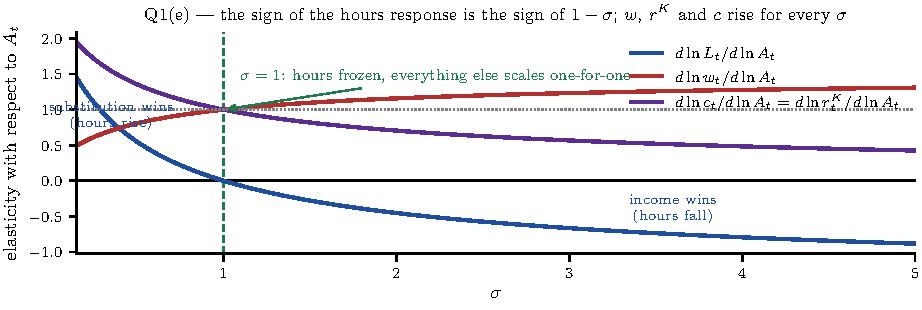
\includegraphics[width=\linewidth]{fig/fig_l5q1_elasticidades.pdf}\\[3pt]
\captionof{figure}{Q1(e). The sign of the hours response is the sign of $1-\sigma$;
$\sigma=1$ is the knife edge, and there everything else scales one-for-one with $A$.}
\label{fig:elas}
\end{center}

\passo{Income and substitution effects.} A rise in $A_t$ raises the marginal product of
labour and therefore the wage. That does two things, and they pull opposite ways.

\begin{itemize}
\item \textbf{Substitution effect.} Leisure is now more expensive --- an hour of leisure
      costs more consumption than before --- so the household substitutes away from leisure
      and \emph{works more}.
\item \textbf{Income effect.} At any given number of hours the household is richer. Leisure
      is a normal good, so it wants more of it and \emph{works less}.
\end{itemize}

\resp{$\sigma$ is the arbiter.} $\sigma$ is how fast the marginal utility of consumption
falls as consumption rises. If $\sigma$ is \textbf{large}, marginal utility collapses
quickly, so the extra consumption the higher wage would buy is not worth much: the
household takes the gain as leisure, the income effect dominates, and hours fall. If
$\sigma$ is \textbf{small}, marginal utility falls slowly, the extra consumption is still
worth having, the substitution effect dominates, and hours rise.

\begin{tcolorbox}[rubricbox]
\small
At $\sigma=1$ \emph{exactly} the two cancel. That is not a coincidence: logarithmic utility
in consumption is the unique case in which income and substitution effects on labour supply
offset one another exactly, which is why it is the standard assumption in growth models
that want hours to be stationary along a balanced growth path.

\smallskip
\textbf{You have already seen this knife edge.} In Problem Set 4, with $\ln c$ and no
transfer, hours were completely independent of the wage and of the tax --- the effect had to
be carried by the lump-sum transfer $T$. Here the same cancellation is what makes
$\sigma=1$ the dividing line. \emph{Same fact, seen twice.}
\end{tcolorbox}

%======================================================================
\section{Question 2 \quad Infinite horizon, labour fixed at $L_t=1$}
%======================================================================

\subsection*{Item (a) --- the household problem and the Euler equation}

\[
\max_{\{c_t,\,a_{t+1}\}}\;\sum_{t=0}^{\infty}\beta^t u(c_t),
\qquad u(c)=\frac{c^{1-\sigma}}{1-\sigma},
\]
subject to the flow budget constraint in every period
\[
a_{t+1}=(1+r_t)a_t+w_t+\Pi_t-c_t ,
\tag{2.1}
\]
with $a_0$ given by the initial capital stock $K_0$, and a \textbf{No-Ponzi condition}
\[
\lim_{T\to\infty}\frac{a_{T+1}}{\prod_{t=0}^{T}(1+r_t)}\;\ge\;0 .
\tag{2.2}
\]
Labour income is $w_t$ because $L_t=1$, and $\Pi_t=0$ by the constant-returns argument of
Question~1(a). \textbf{Say explicitly why (2.2) is needed}: without it the household would
roll debt over forever, financing unbounded consumption, and the problem would have no
solution.

\passo{The Euler equation, by a perturbation.} Cut $c_t$ by $\varepsilon$ and save the
proceeds. Utility cost today: $u'(c_t)\varepsilon$. The $\varepsilon$ becomes
$(1+r_{t+1})\varepsilon$ tomorrow, worth
$\beta(1+r_{t+1})u'(c_{t+1})\varepsilon$ in today's units. At an optimum no such
perturbation can help:
\[
\boxed{\;u'(c_t)=\beta(1+r_{t+1})\,u'(c_{t+1})\;}
\qquad\Longleftrightarrow\qquad
\boxed{\;\frac{c_{t+1}}{c_t}=\big[\beta(1+r_{t+1})\big]^{1/\sigma}\;}
\tag{2.3}
\]

\intuicao{The Euler equation is a no-arbitrage condition on the household's \emph{own}
consumption plan. The left side is the marginal cost of giving up a unit today; the right
side is the marginal benefit, discounted because tomorrow matters less.}

\passo{The same result with multipliers --- and what $\lambda_t$ is here.} The perturbation
argument is the fastest route, but it is worth seeing the Lagrangian once, because the
multiplier changes character relative to Question~1. There is now \textbf{one constraint
per date}, so there is one multiplier per date:
\[
\mathcal{L}=\sum_{t=0}^{\infty}\Big\{\beta^t u(c_t)
+\lambda_t\big[(1+r_t)a_t+w_t+\Pi_t-c_t-a_{t+1}\big]\Big\}
\]
Two first-order conditions. In $c_t$, and in $a_{t+1}$ --- which appears with a minus sign
in the date-$t$ constraint and inside $(1+r_{t+1})a_{t+1}$ in the date-$(t+1)$ one:
\[
\frac{\partial\mathcal{L}}{\partial c_t}:\quad \beta^t u'(c_t)=\lambda_t ,
\qquad\qquad
\frac{\partial\mathcal{L}}{\partial a_{t+1}}:\quad \lambda_t=\lambda_{t+1}(1+r_{t+1}).
\]
Substituting the first into the second, $\beta^t
u'(c_t)=\beta^{t+1}u'(c_{t+1})(1+r_{t+1})$, and dividing by $\beta^t$ returns (2.3)
exactly. \checkmark

\smallskip
Here $\lambda_t=\beta^t u'(c_t)$ is the \textbf{discounted} marginal utility of date-$t$
consumption: the value, measured in date-0 utils, of handing the household one more good at
date $t$. The second condition says $\lambda_t/\lambda_{t+1}=1+r_{t+1}$ --- the multipliers
fall through time at exactly the interest rate, because that is the rate at which goods can
be moved. In Question~1 the two dates had already been merged into a single constraint, so
a single $\lambda$ did this job; the ratio $\lambda_t/\lambda_0=1/\prod_{s\le
t}(1+r_s)$ is the same object as the $\tfrac{1}{1+r}$ that sat inside (1.1). \emph{Same
economics, two bookkeeping conventions.}

\passo{The condition that closes the problem.} The Euler equation is necessary, not
sufficient: it fixes the \emph{slope} of the consumption path and says nothing about its
\emph{level}. What pins the level down is the \textbf{transversality condition}
\[
\lim_{T\to\infty}\beta^T u'(c_T)\,a_{T+1}=0 .
\tag{2.3'}
\]
Read it together with No-Ponzi (2.2): the household may not die in debt (2.2), and it must
not die holding assets of positive present value either, since consuming them would raise
utility at no cost (2.3$'$). Between them: \textbf{spend everything, eventually.} This is
the infinite-horizon counterpart of the step in Question~1(a) where the date-2 constraint
was imposed with equality because there was no date~3.

\passo{What makes consumption grow.} From (2.3), $c_{t+1}>c_t$ if and only if
$\beta(1+r_{t+1})>1$, that is
\[
\boxed{\;r_{t+1}>\tfrac{1}{\beta}-1\equiv\rho\;}
\]
\resp{Consumption grows exactly when the market's reward for waiting exceeds the
household's impatience.} When it does not, the path slopes down.

\passo{The role of $\sigma$.} It enters only through the exponent $1/\sigma$, which is the
\textbf{elasticity of intertemporal substitution}. It governs how strongly the household
tilts its path for a \emph{given} gap between $r$ and $\rho$. High $\sigma$ means low
elasticity: the household strongly resists letting consumption differ across dates, so even
a large gap produces only a gentle slope.

\begin{tcolorbox}[trapbox, title={What $\sigma$ does \emph{not} do}]
\small
$\sigma$ affects only \textbf{how fast} the economy travels, never \textbf{where it ends
up}. It vanishes from the steady-state condition in item (d) --- setting $c_{t+1}/c_t=1$
raises the bracket to the power $1/\sigma$, and $1^{1/\sigma}=1$ for any $\sigma$.
\checkmark\ (verified for $\sigma\in\{0{,}5;\,1;\,2;\,3;\,8\}$ in
\texttt{l5q2.py::check\_estado\_estacionario}.)
\end{tcolorbox}

\subsection*{Item (b) --- the firm's problem and factor prices}

\[
\max_{K_t,\,L_t}\;\;A K_t^{\alpha}L_t^{1-\alpha}-w_tL_t-r^K_tK_t
\]
First-order conditions, evaluated at $L_t=1$:
\[
\boxed{\;w_t=(1-\alpha)A K_t^{\alpha}\;},
\qquad
\boxed{\;r^K_t=\alpha A K_t^{\alpha-1}\;}
\tag{2.4}
\]
The wage is \emph{increasing} in the capital stock and the rental rate \emph{decreasing} in
it --- both by diminishing returns: more capital per worker raises the marginal product of
labour and lowers the marginal product of capital. Profits are zero, so household income is
wages plus capital income and nothing else.

\subsection*{Item (c) --- who owns the capital, and why it does not matter}

\passo{Arrangement (i): the household owns $K$, rents it out, and invests itself.}
Its budget constraint is
\[
c_t+I_t=w_t+r^K_tK_t,
\qquad
K_{t+1}=(1-\delta)K_t+I_t .
\]
Substitute $I_t=K_{t+1}-(1-\delta)K_t$ out and collect the $K_t$ terms:
\[
c_t+K_{t+1}=w_t+\underbrace{\big(r^K_t+1-\delta\big)}_{\text{gross return on capital}}K_t .
\tag{2.5}
\]
The bracket is the point: a unit of capital carried into date $t$ pays its rent $r^K_t$
\emph{and} survives as $1-\delta$ units of machine, so its gross return is the sum of the
two. That is already the whole of (2.7) in embryo --- a bond carried into date $t$ pays
$1+r_t$, and nothing distinguishes the two but the label.

\smallskip
Now derive the condition instead of quoting it. Solve (2.5) for $c_t$,
\[
c_t=w_t+\big(r^K_t+1-\delta\big)K_t-K_{t+1},
\]
and substitute into the objective, so that the household is choosing the \emph{sequence}
$\{K_{t+1}\}$ directly. Each $K_{t+1}$ then appears in exactly \textbf{two} terms of
$\sum_s\beta^s u(c_s)$: at date $t$, where raising it costs consumption one-for-one, and at
date $t+1$, where it pays the gross return. Hence
\[
\frac{\partial}{\partial K_{t+1}}\sum_{s}\beta^s u(c_s)
=\beta^t u'(c_t)\cdot(-1)+\beta^{t+1}u'(c_{t+1})\big(r^K_{t+1}+1-\delta\big)=0 ,
\]
and dividing through by $\beta^t$:
\[
-u'(c_t)+\beta\,u'(c_{t+1})\big(r^K_{t+1}+1-\delta\big)=0
\quad\Longrightarrow\quad
u'(c_t)=\beta\big(r^K_{t+1}+1-\delta\big)u'(c_{t+1}).
\tag{2.6}
\]
If the household holds bonds \emph{as well}, its constraint is
$c_t+a_{t+1}+K_{t+1}=w_t+(1+r_t)a_t+(r^K_t+1-\delta)K_t$, and the same exercise in
$a_{t+1}$ returns (2.3). Both assets are held in equilibrium, so both must offer the same
return --- otherwise the household would take an unbounded long position in one and short
the other, and no equilibrium would exist. Comparing (2.6) with the bond Euler equation
(2.3), the marginal utilities cancel and:
\[
\boxed{\;1+r_{t+1}=r^K_{t+1}+1-\delta\;}
\tag{2.7}
\]

\passo{Arrangement (ii): a separate investment firm.} Its profit is Kurlat (9.3.3):
\[
\Pi^I_t=\max_{I}\;\frac{r^K_{t+1}+1-\delta}{1+r_{t+1}}\big[(1-\delta)K_t+I\big]
-\big[(1-\delta)K_t+I\big].
\]
Differentiate:
\[
\frac{\partial \Pi^I_t}{\partial I}=\frac{r^K_{t+1}+1-\delta}{1+r_{t+1}}-1 ,
\]
which is a \textbf{constant}: the problem is \emph{linear} in $I$ and has no interior
optimum. Three cases, and only one survives:

\begin{center}
\small
\begin{tabular}{@{}lll@{}}
\toprule
Case & What the firm does & Consistent with equilibrium? \\
\midrule
ratio $>1$ & $I\to+\infty$, infinite profit & No --- infinite capital \\
ratio $<1$ & $I\to-\infty$ & No \\
ratio $=1$ & \textbf{any} $I$, profit exactly zero & \textbf{Yes} \\
\bottomrule
\end{tabular}
\end{center}

Setting the ratio to one gives (2.7) again. \resp{The identical condition.} \checkmark\
(both routes, plus the linearity claim itself, in \texttt{l5q2.py::check\_arbitragem}).

\begin{tcolorbox}[trapbox, title={The subtlety almost everyone gets wrong}]
\small
The investment firm's first-order condition \textbf{does not determine how much is
invested}. It determines a \textbf{price}. At the no-arbitrage return the firm is genuinely
indifferent across every level of $I$, so the quantity of investment must come from
somewhere else --- namely \textbf{goods market clearing}, item (d). Looking for ``the
investment firm's optimal $I$'' is looking for something that does not exist.
\end{tcolorbox}

\passo{Why the allocation does not depend on who owns the capital.} Three reasons; give all
three.

\begin{enumerate}[label=\textbf{\arabic*.}, leftmargin=2em]
\item \textbf{The same intertemporal price.} Both arrangements deliver (2.7), so the
      household faces the same trade-off between a unit of consumption today and one
      tomorrow, whether it holds the claim as physical capital or as a bond. The rate at
      which the \emph{economy} can move goods through time is a technological fact; the
      no-arbitrage condition just makes the financial price match it.
\item \textbf{Zero profits in both.} The productive firm earns zero by constant returns; the
      investment firm earns zero because that is precisely what (2.7) enforces. No
      arrangement transfers any surplus to anybody, so the household's lifetime budget set
      is \emph{identical}.
\item \textbf{Nothing real has moved.} Consumption possibilities depend only on the
      economy's resource constraint and on the intertemporal price, and ownership touches
      neither.
\end{enumerate}

\intuicao{This is \textbf{Fisher separation} (Fisher, \emph{The Theory of Interest}, 1930),
and it has the same flavour as Modigliani--Miller: with complete and competitive markets,
how a claim on a real asset is packaged does not change real outcomes. In one sentence: the
investment firm is an \emph{accounting device}, not an agent with independent influence,
because arbitrage strips it of any profit and hands the entire intertemporal trade-off back
to the household unchanged.}

\subsection*{Item (d) --- resource constraint, steady state, closed forms}

\passo{The resource constraint.} Goods market clearing with $L_t=1$ is
$A K_t^{\alpha}=c_t+I_t$; capital accumulation is $K_{t+1}=(1-\delta)K_t+I_t$. Substituting
$I_t$ out:
\[
\boxed{\;K_{t+1}=(1-\delta)K_t+A K_t^{\alpha}-c_t\;}
\tag{2.8}
\]
In words: the capital you carry into tomorrow is what survives depreciation, plus everything
you produced, minus everything you ate. Together with (2.3) this is a pair of difference
equations in $(K_t,c_t)$, and from here everything is geometry.

\passo{The steady state.} Constant consumption in (2.3) requires $\beta(1+r)=1$, so
$1+r=1/\beta$. Combining with the arbitrage condition (2.7) and the firm's condition (2.4),
$r=r^K-\delta=F_K(K,1)-\delta$:
\[
\boxed{\;F_K(K\stst,1)-\delta=\frac{1}{\beta}-1\;}
\tag{2.9}
\]
which is what the question asks you to show, and is Kurlat (9.3.17).

\passo{Closed forms.} With $F_K=\alpha A K^{\alpha-1}$:
\[
\alpha A (K\stst)^{\alpha-1}=\frac{1}{\beta}-1+\delta
\qquad\Longrightarrow\qquad
\boxed{\;K\stst=\left[\frac{\alpha A}{\frac{1}{\beta}-1+\delta}\right]^{\frac{1}{1-\alpha}}
=\left[\frac{\alpha A\beta}{1-\beta+\beta\delta}\right]^{\frac{1}{1-\alpha}}\;}
\tag{2.10}
\]
and setting $K_{t+1}=K_t$ in (2.8):
\[
\boxed{\;c\stst=A\,(K\stst)^{\alpha}-\delta K\stst\;}
\tag{2.11}
\]
--- output minus replacement investment. In a steady state \emph{all} investment is
replacement investment.

\checkmark\ Both verified as a genuine rest point of (2.3) and (2.8), for four values of
$\beta$ and five of $\sigma$.

\passo{The steady-state interest rate.}
\[
\boxed{\;r\stst=\frac{1}{\beta}-1=\rho\;}
\]
\resp{It depends on $\beta$ and on nothing else} --- not on $A$, not on $\alpha$, not on
$\delta$.

\begin{tcolorbox}[planbox, title={Why --- and this is the punchline of the question}]
\small
In a steady state consumption is constant, and the Euler equation says a constant path
requires $\beta(1+r)=1$ \emph{exactly}. That is a statement purely about \textbf{preferences}:
the reward for waiting must precisely offset impatience, which is the only configuration
under which the household is content to consume the same amount forever. Technology has no
say in it.

\smallskip
What technology determines is the \textbf{quantity} of capital. Given that $r$ must equal
$1/\beta-1$, the capital stock adjusts until $F_K-\delta$ matches that number. A more
productive economy does not end up with a higher interest rate; it ends up with
\textbf{more capital}, which drives $F_K$ back down until it meets what preferences demand.

\smallskip
\resp{Preferences determine the interest rate; technology determines the capital stock.}
Say it in exactly those words.
\end{tcolorbox}

\passo{The numbers.} $A=1$, $\alpha=0{,}35$, $\delta=0{,}08$:

\begin{center}
\small
\begin{tabular}{@{}rrrrrr@{}}
\toprule
$\beta$ & $K\stst$ & $c\stst$ & $F_K-\delta$ & $r\stst$ & $K\stst/K_{gr}$ \\
\midrule
0,900 & 2,53676 & 1,18221 & $0{,}11111$ & $11{,}11\%$ & 0,262 \\
0,960 & 5,08153 & 1,35991 & $0{,}04167$ & $4{,}17\%$ & 0,525 \\
0,990 & 8,06630 & 1,43122 & $0{,}01010$ & $1{,}01\%$ & 0,833 \\
0,999 & 9,50193 & 1,43889 & $0{,}00100$ & $0{,}10\%$ & 0,981 \\
\bottomrule
\end{tabular}
\end{center}

Moving $\beta$ from $0{,}90$ to $0{,}99$ --- a change in impatience of about ten percentage
points a year --- \textbf{more than triples} the steady-state capital stock. Patience is
enormously powerful for capital. Consumption, however, moves only from $1{,}18$ to $1{,}43$,
about $21\%$. Item (e) explains that asymmetry.

\begin{center}
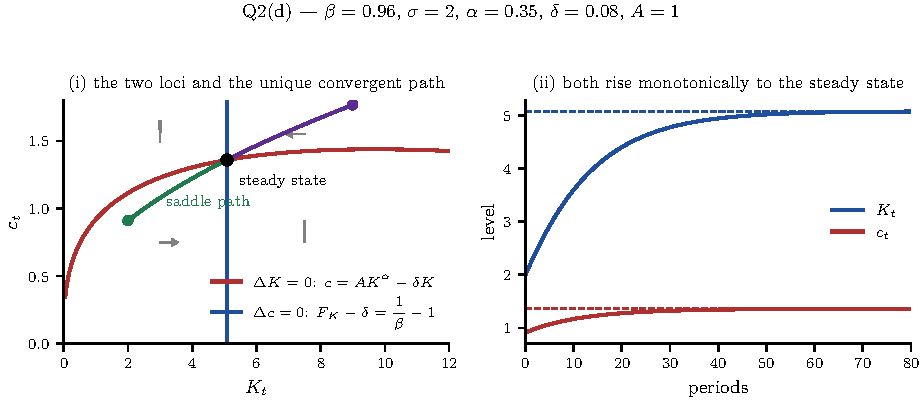
\includegraphics[width=\linewidth]{fig/fig_l5q2_fase.pdf}\\[3pt]
\captionof{figure}{Q2(d). Left: the $\Delta c=0$ locus is \emph{vertical} because $c$ does
not appear in (2.9); the $\Delta K=0$ locus is the concave hump $c=AK^{\alpha}-\delta K$.
Only one trajectory converges --- the saddle path. Right: the same transition against time.
$K$ is a \emph{state} variable and cannot jump; $c$ is a \emph{jump} variable and must.}
\label{fig:fase}
\end{center}

\subsection*{Item (e) --- Bonus: the Golden Rule}

\passo{Derivation.} The Golden Rule maximises steady-state consumption. From (2.11),
maximise $A K^{\alpha}-\delta K$ over $K$:
\[
\alpha A K^{\alpha-1}-\delta=0
\qquad\Longrightarrow\qquad
\boxed{\;F_K(K_{gr},1)=\delta\;},
\qquad
\boxed{\;K_{gr}=\left(\frac{\alpha A}{\delta}\right)^{\frac{1}{1-\alpha}}\;}
\tag{2.12}
\]
\checkmark\ (confirmed as the argmax of $c\stst(K)$ on a grid of $6\times10^5$ points).

\passo{The comparison.} Put the two conditions side by side:
\[
\text{Golden Rule:}\quad F_K=\delta
\qquad\text{vs}\qquad
\text{competitive steady state:}\quad F_K=\delta+\underbrace{\Big(\tfrac{1}{\beta}-1\Big)}_{>\,0\ \text{iff}\ \beta<1} .
\]
Since $\beta<1$, the marginal product of capital at the competitive steady state is
\textbf{strictly greater} than at the Golden Rule. And $F_K$ is strictly \emph{decreasing}
in $K$. Therefore
\[
\boxed{\;K\stst<K_{gr}\;}
\]
With the calibration above, $K_{gr}=9{,}685$ and $c_{gr}=1{,}43898$, so at $\beta=0{,}96$
the economy holds only $52\%$ of the Golden Rule capital stock. \checkmark

\passo{Why an efficient economy stops short.} The First Welfare Theorem says the
competitive equilibrium is Pareto efficient. So why not accumulate ``enough''?

\begin{enumerate}[label=\textbf{\arabic*.}, leftmargin=2em]
\item \textbf{Reject the premise hidden in ``enough''.} The Golden Rule maximises
      consumption \emph{in the steady state}. It says nothing about the path taken to get
      there and gives no weight at all to \emph{when} consumption arrives. It is a criterion
      about one point, not about a trajectory.
\item \textbf{Say what the household actually maximises.} The household maximises the
      \emph{discounted} sum of utility over the whole path. Moving from $K\stst$ up to
      $K_{gr}$ requires investing more --- consuming \emph{less} --- for a long stretch, in
      exchange for higher consumption in the far future. An impatient household discounts
      that far-future gain and ranks the whole package \emph{below} where it already is.
\item \textbf{Conclude sharply.} \resp{Under-accumulation relative to the Golden Rule is not
      a market failure. It is the optimum.} There is no Pareto improvement available ---
      which is exactly what the First Welfare Theorem asserts --- and the reason there is
      none is that reaching the Golden Rule would demand a sacrifice today that the
      household does not want to make. \textbf{The Golden Rule is a benchmark, not a
      target}; it stops being normative the moment somebody in the model has preferences.
\end{enumerate}

\begin{tcolorbox}[rubricbox, title={The contrast that makes the point}]
\small
In the \textbf{Solow} model with an \emph{exogenous} saving rate the economy can perfectly
well end up on the \emph{other} side, with $K>K_{gr}$. That is \textbf{dynamic
inefficiency}, and it is a genuine failure: consumption could be raised in every period,
starting immediately, simply by saving less. Kurlat's Exercise \textbf{6.7} (p.~124)
constructs exactly that case, with $s=0{,}4$ against $\alpha=0{,}35$, producing a negative
real interest rate.

\smallskip
What the present model shows is that dynamic inefficiency \textbf{can never happen} once the
saving rate is \emph{chosen} rather than assumed. An optimising household would never
over-accumulate. Only an exogenous saving rate can produce that pathology.
\end{tcolorbox}

\passo{The limit as $\beta\to1$.} As $\beta\to1$, $\frac{1}{\beta}-1\to0$, so (2.9)
converges to $F_K=\delta$, which is precisely (2.12). Hence
\[
\boxed{\;\beta\to1\;\Longrightarrow\;K\stst\to K_{gr}\;}
\]
\checkmark\ At $\beta=1-10^{-9}$ the ratio $K\stst/K_{gr}$ is $1$ to six decimal places.
\resp{The distance between the competitive steady state and the Golden Rule \emph{is}
impatience, measured.}

\begin{center}
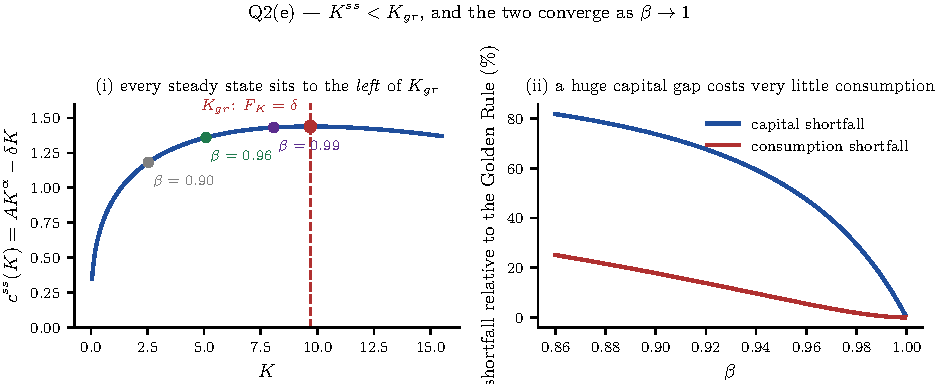
\includegraphics[width=\linewidth]{fig/fig_l5q2_regradeouro.pdf}\\[3pt]
\captionof{figure}{Q2(e). Left: every steady state lies to the left of $K_{gr}$, and slides
toward it as $\beta$ rises. Right: the two shortfalls. Because $c\stst(K)$ is at a maximum
at $K_{gr}$, its first derivative there is zero and the consumption loss is
\emph{second order}.}
\label{fig:gr}
\end{center}

\begin{tcolorbox}[planbox, title={One observation worth adding, and most students miss it}]
\small
At $\beta=0{,}999$ the capital stock is $1{,}9\%$ short of the Golden Rule, but consumption
is short by only \textbf{0,006\%}. Even at $\beta=0{,}96$, where capital is barely half the
Golden Rule level, consumption is only $5{,}5\%$ below.

\smallskip
The reason is that $K_{gr}$ is a \emph{maximum}, so $c\stst(K)$ is flat there: the first
derivative vanishes and the loss from being off the peak is \textbf{second order}. Two
consequences. First, arguments that an economy is losing a lot of consumption by
under-accumulating are usually quantitatively weak. Second, this is the same flatness that
makes Kurlat's Exercise \textbf{9.12} (p.~185) come out as it does, where optimising the
entire savings path for 150 years is worth about a third of one percent of consumption
relative to using the correct constant rate.
\end{tcolorbox}

%======================================================================
\section*{Companion code}
\addcontentsline{toc}{section}{Companion code}
%======================================================================

Every number above is reproduced by \texttt{Resolucao/lista5\_codigo/}. Each script checks
its analytical formulas against an independent numerical route and \textbf{aborts on any
mismatch}.

\begin{center}
\small
\begin{tabular}{@{}lp{10.4cm}@{}}
\toprule
\textbf{File} & \textbf{What it does} \\
\midrule
\texttt{modelo.py} & Every closed form, once: Q1's two equivalent forms of the labour
equation, the elasticities, the interest rate; Q2's steady state, Golden Rule, the two
difference equations, and a bisection that shoots for the saddle path. \\
\texttt{l5q1.py} & Zero profit via Euler's theorem; the raw and tidied labour equations share
the same unique root for 5 values of $\sigma$ and 4 of $A$; the LHS of (1.8) is strictly
increasing on a $2\times10^5$-point grid; (1.10) against a symmetric finite difference, and
the induced elasticities of $w$, $r^K$ and $c$ against their own; $r^K=\alpha c/\Kb$
exactly; and the interest rate, including the $A_2=A_1$ collapse to $1/\beta-1$. \\
\texttt{l5q2.py} & Both ownership routes give the same $r$, and the investment firm's profit
is identically zero in $I$ at that $r$ and strictly monotone at any other; the steady state
is a rest point for every $\sigma$; $K\stst<K_{gr}$; $K_{gr}$ is the argmax of $c\stst$;
$K\stst\to K_{gr}$ as $\beta\to1$; and the saddle path converges while neighbouring paths
fall off it in both directions. \\
\texttt{l5\_figuras.py} & The four figures. \\
\texttt{estilo\_mpl.py} & \texttt{pgf} backend, so figure text is typeset by
\texttt{pdflatex} with \texttt{lmodern} and \texttt{cmap} and the PDF stays fully copyable. \\
\bottomrule
\end{tabular}
\end{center}

\end{document}
